\section{Variational Autoencoders - VAEs}
\label{VAEs}

Based on the seminal work by \citeauthor{diggleImplicitPrescribed}, generative models can be classified into two broad categories. Prescribed models employ a well-defined, often parametric, mathematical expression for the probability density function (pdf), which enables easier analytical interpretation of the distributions. In contrast, implicit models synthesize new data samples without relying on an explicit pdf, approximating the underlying data distribution on which they were trained \citep{diggleImplicitPrescribed}. Variational Autoencoders (VAEs), which inherit the foundational architecture of autoencoders, belong to the prescribed models category as they require an explicit formulation of the probability density function (pdf) to function effectively. This feature makes VAEs suitable for tasks that require not only the generation but also the understanding of complex data distributions. \citep{kingmaVAE,rezendeVAE,GoodfellowDeepLearning}. Generative Adversarial Networks (GANs) \citep{goodfellowGAN}, discussed later, are a prime example ofthe latter category.

VAEs inherit the fundamental architecture of autoencoders, consisting of an encoder and a decoder. The encoder aims to transform the input data into a lower-dimensional latent space representation (vector), often referred to as the "code" or "bottleneck" \citep{hintonCode, GoodfellowDeepLearning}. This code captures the most relevant features of the input while reducing its dimensionality. The decoder then reconstructs the original input data from the given latent vector using a loss function. However, the core objective of an autoencoder is not the reconstruction itself but the extraction of a meaningful latent vector \citep{GoodfellowDeepLearning}, which serves as a simplified representation of the input."Autoencoders have been successfully applied to dimensionality reduction and information retrieval tasks." \citep{GoodfellowDeepLearning}. The ability to reduce dimensionality has practical implications for improving the efficiency of classification tasks by reducing computational and memory overhead \citep{GoodfellowDeepLearning}. When paired with information retrieval, this dimensionality reduction makes searching in certain low-dimensional spaces particularly efficient \citep{GoodfellowDeepLearning}. Despite these advantages, autoencoders are not designed to generate new data; their main function is to copy and reconstruct the given input \citep{GoodfellowDeepLearning}.

\textcolor{blue}{while similiar inputs tend to cluster in similiar latent spaces.
It can be seen that the same digits tend to cluster themselves in the latent space. Another important thing to note is that there are parts of the latent space that doesn't correspond to any data point. Using those as inputs to the encoder will result in an output that doesn’t look like any digit from the MNIST data. This is what we mean by that the latent space is not regularized. Such a latent space only has a few regions/cluster that has the generative capability, which means that sampling any point in the latent space that belongs within a cluster will generate a variation of the data that the cluster belongs to. But the entire latent space does not have the generative capability. The regions which do not belong to any cluster will generate garbage output. Once the network is trained, and the training data is removed, we have no way of knowing if the output generated by the decoder from a randomly sampled latent vector is valid or not. Hence AE is mainly used for compression - https://towardsdatascience.com/difference-between-autoencoder-ae-and-variational-autoencoder-vae-ed7be1c038f2}


\begin{figure}[ht]
    \centering
      \hspace{.8cm}
      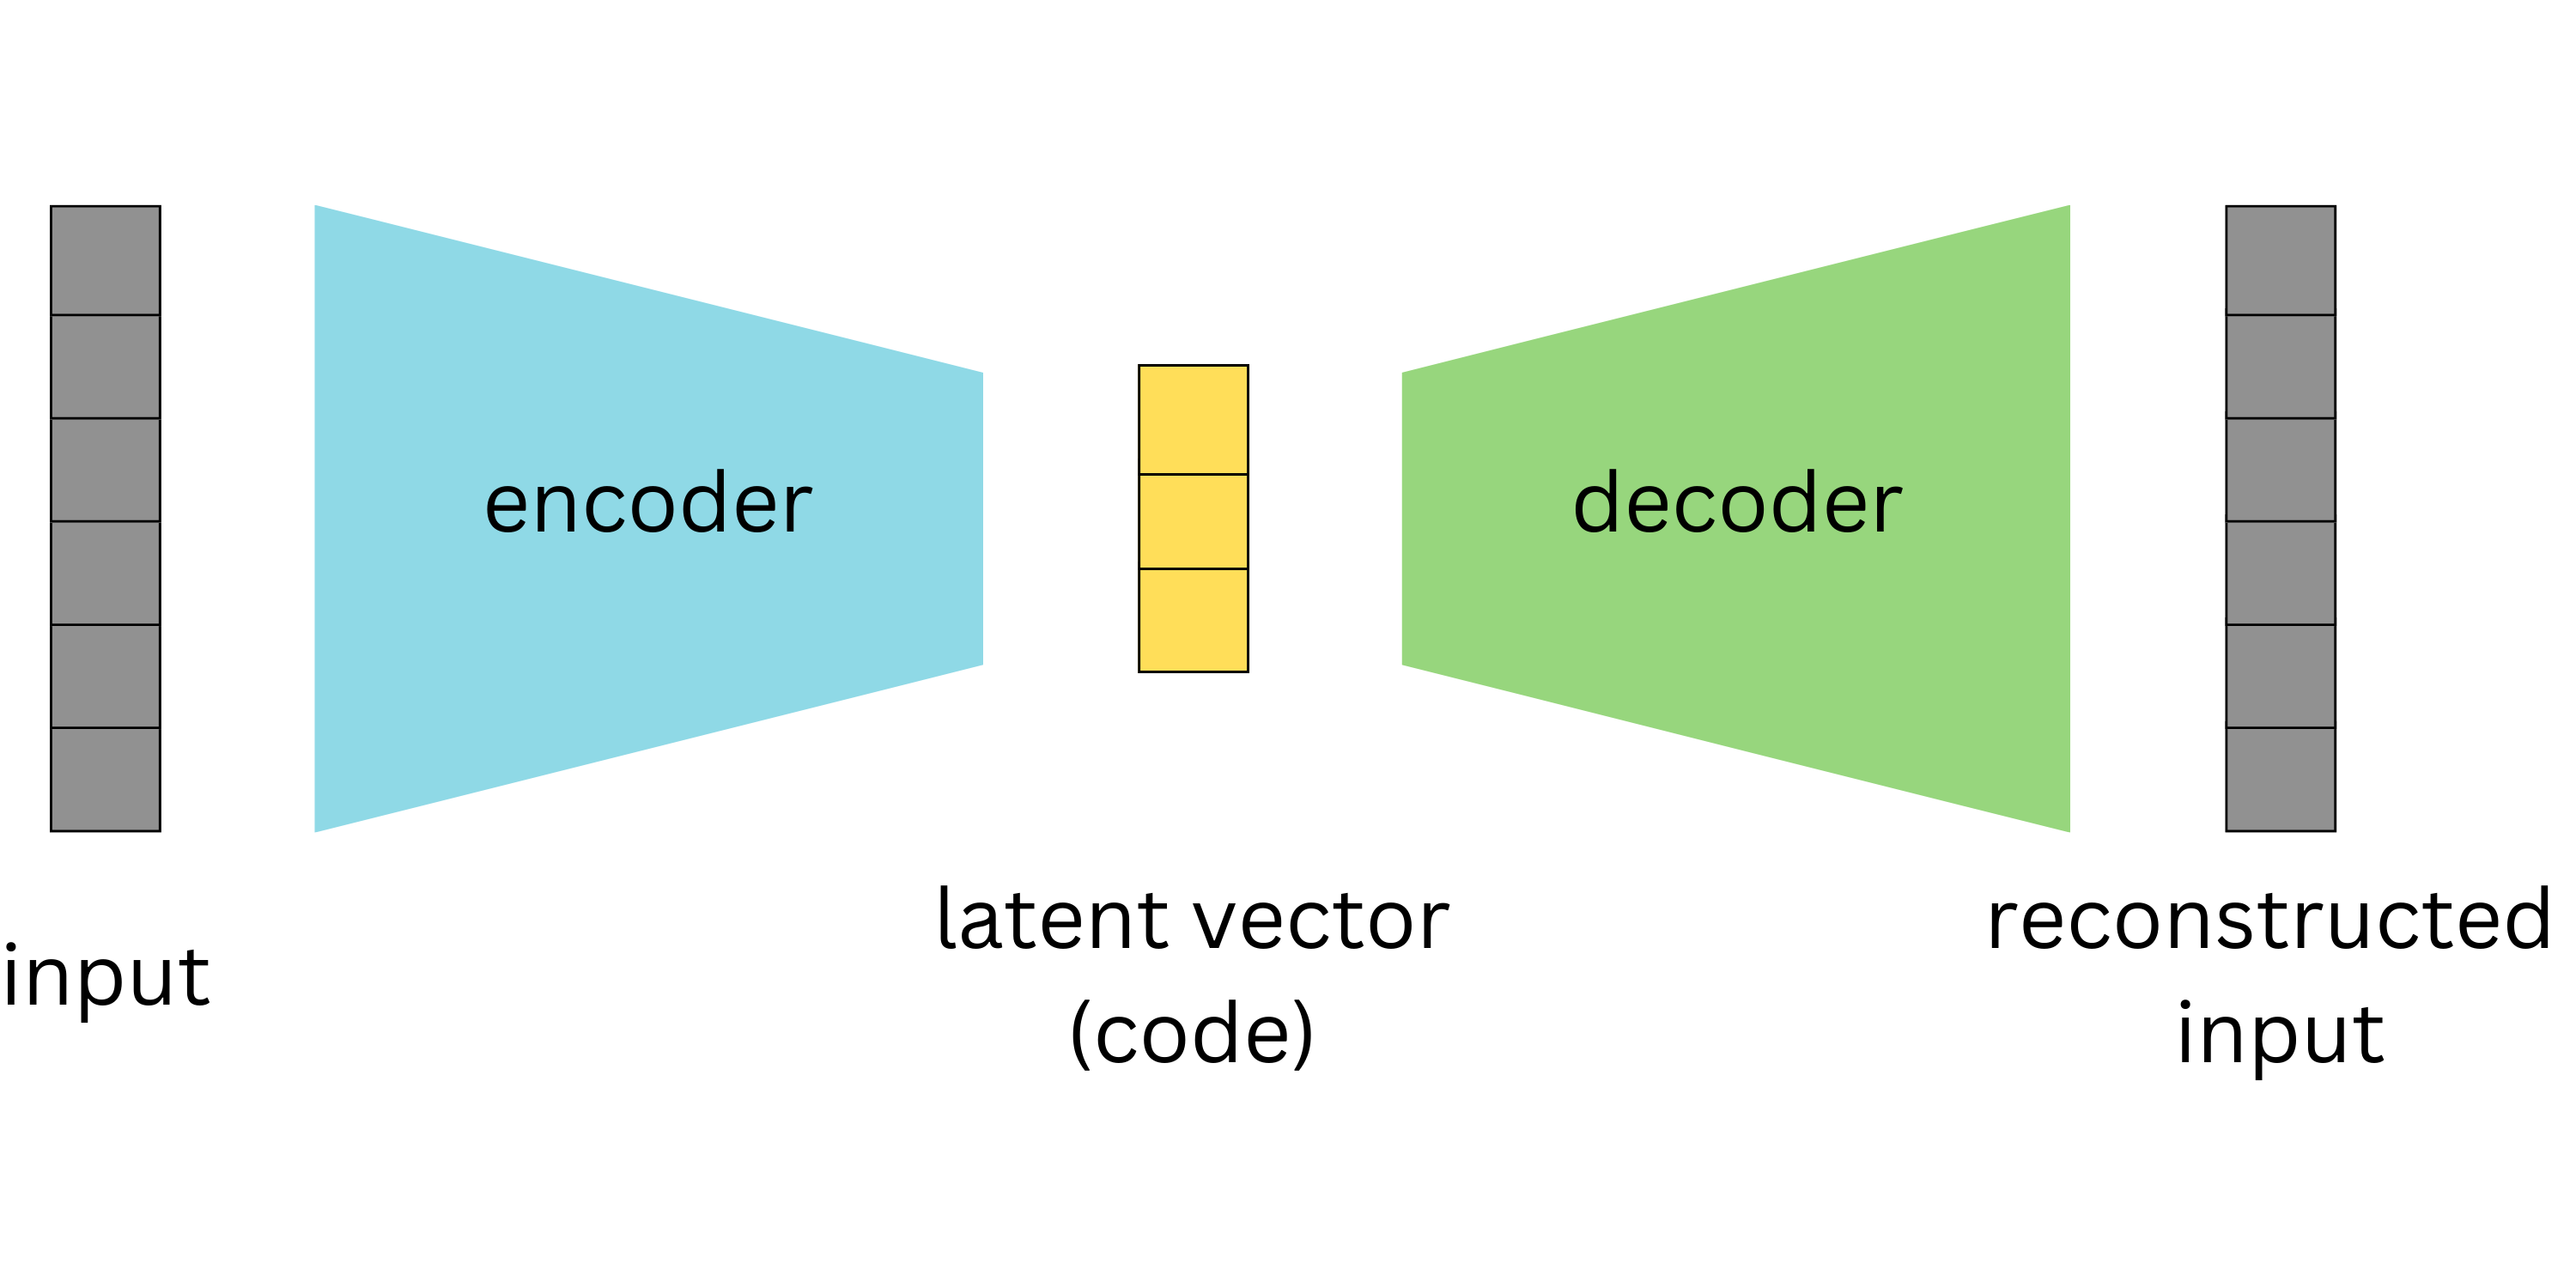
\includegraphics[width=.7\columnwidth]{figures/Autoencoder.png}
      \caption{Autoencoder: The encoder reduces the input dimension to a latent vector that captures the most important features. The decoder then uses this vector to reconstruct the input, with training aimed at minimizing reconstruction loss.}
      \label{fig:figureAE}
    \end{figure}

In VAEs, the encoder compresses the input into a latent variable space and creates a probability distribution over the latent variables. This allows for robustness against overfitting and enables the model to synthesize new, analogous data points by sampling from this distribution and subsequent decoding \citep{kingmaVAE, rezendeVAE}.During the training phase, VAEs identify specific regions in the latent variable space, akin to "pools," for different categories of data, such as various types of animals. These regions enable VAEs to overcome a limitation inherent in standard autoencoders—the uncertainty of where to sample a useful latent vector for the decoder. In VAEs, this uncertainty is mitigated by constraining the latent space to known regions from which vectors can be confidently sampled \citep{doerschVAE}. The decoder in VAEs reconstructs the original input or synthesizes new outputs from sampled latent variables, optimized via a loss function that considers both reconstruction loss and a regularization term based on the Kullback-Leibler (KL) divergence \citep{GoodfellowDeepLearning}. This divergence measures differences between the estimated and true data distributions \citep{kingmaVAE}, aiding the model in generalizing effectively to unseen data


\begin{figure}[ht]
    \centering
      \hspace{.8cm}
      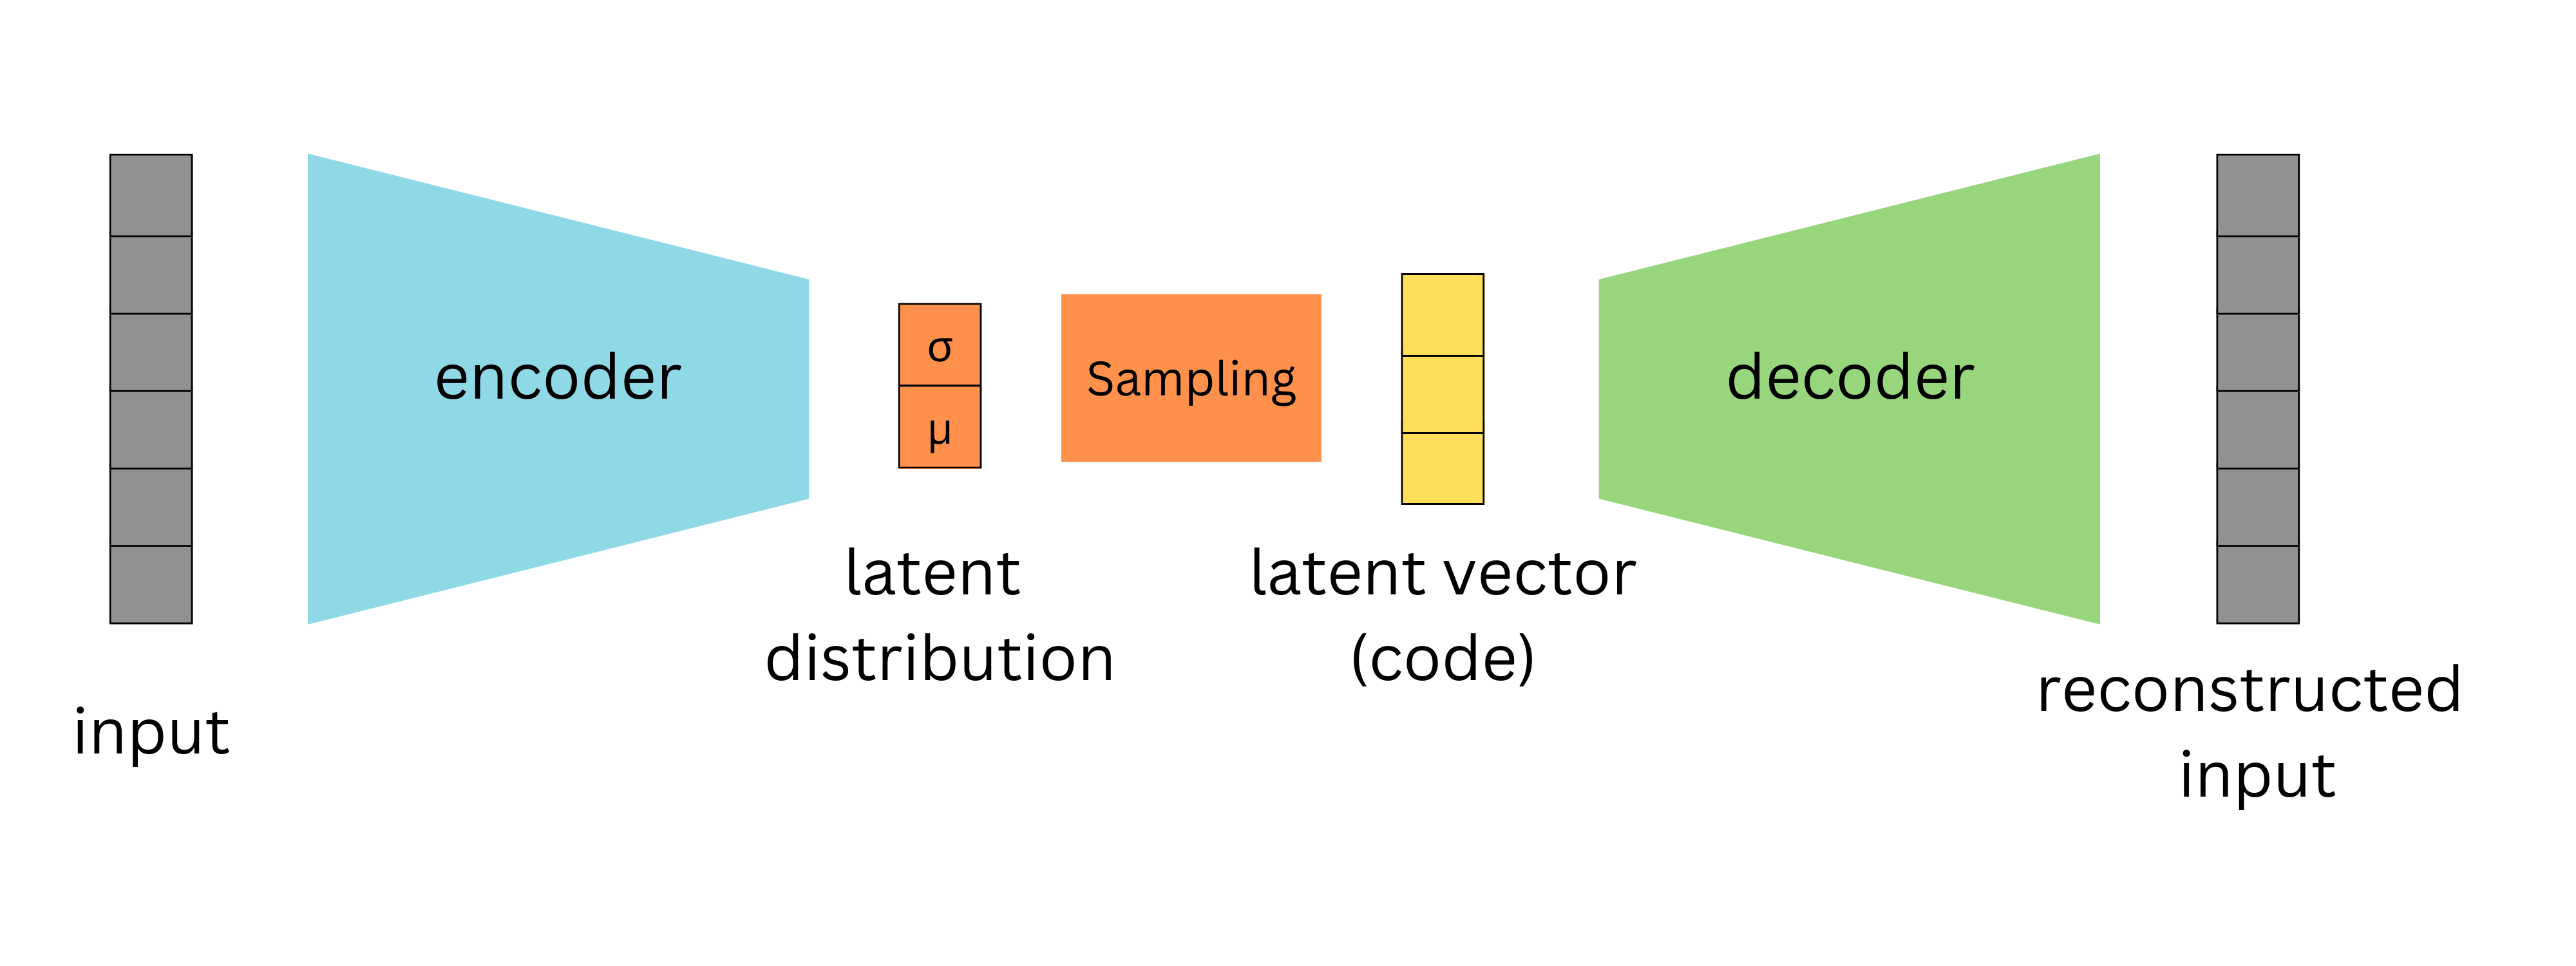
\includegraphics[width=.9\columnwidth]{figures/VAE.png}
      \caption{Functionality of a Variational Autoencoder, demonstrating incorporation of mean and standard deviation for enhancing generative capabilities.}
      \label{fig:figureVAE}
\end{figure}

Despite their capabilities, VAEs exhibit some limitations. According to \citeauthor{GoodfellowDeepLearning}, the generated samples can often be blurry. He explains that the blurriness observed may be due to their optimization process, which minimizes Kullback-Leibler divergence. This could lead the model to assign high probabilities to blurry images. The Gaussian distribution often used in VAEs for the generative model may also contribute to this effect, as it can ignore minor features in the input data \citep{GoodfellowDeepLearning}. Another issue is that VAEs typically utilize only a small portion of the latent space, which might further compromise the quality of generated images \citep{GoodfellowDeepLearning}. The performance of the model is also sensitive to the choice of priors for the latent space, making hyperparameter tuning an essential aspect of working with VAEs \citep{kingmaVAE, higginsVAE}. 